\section{Knowledge base generator}
\label{knowledge base generator}
\begin{figure}[htp]
\centering
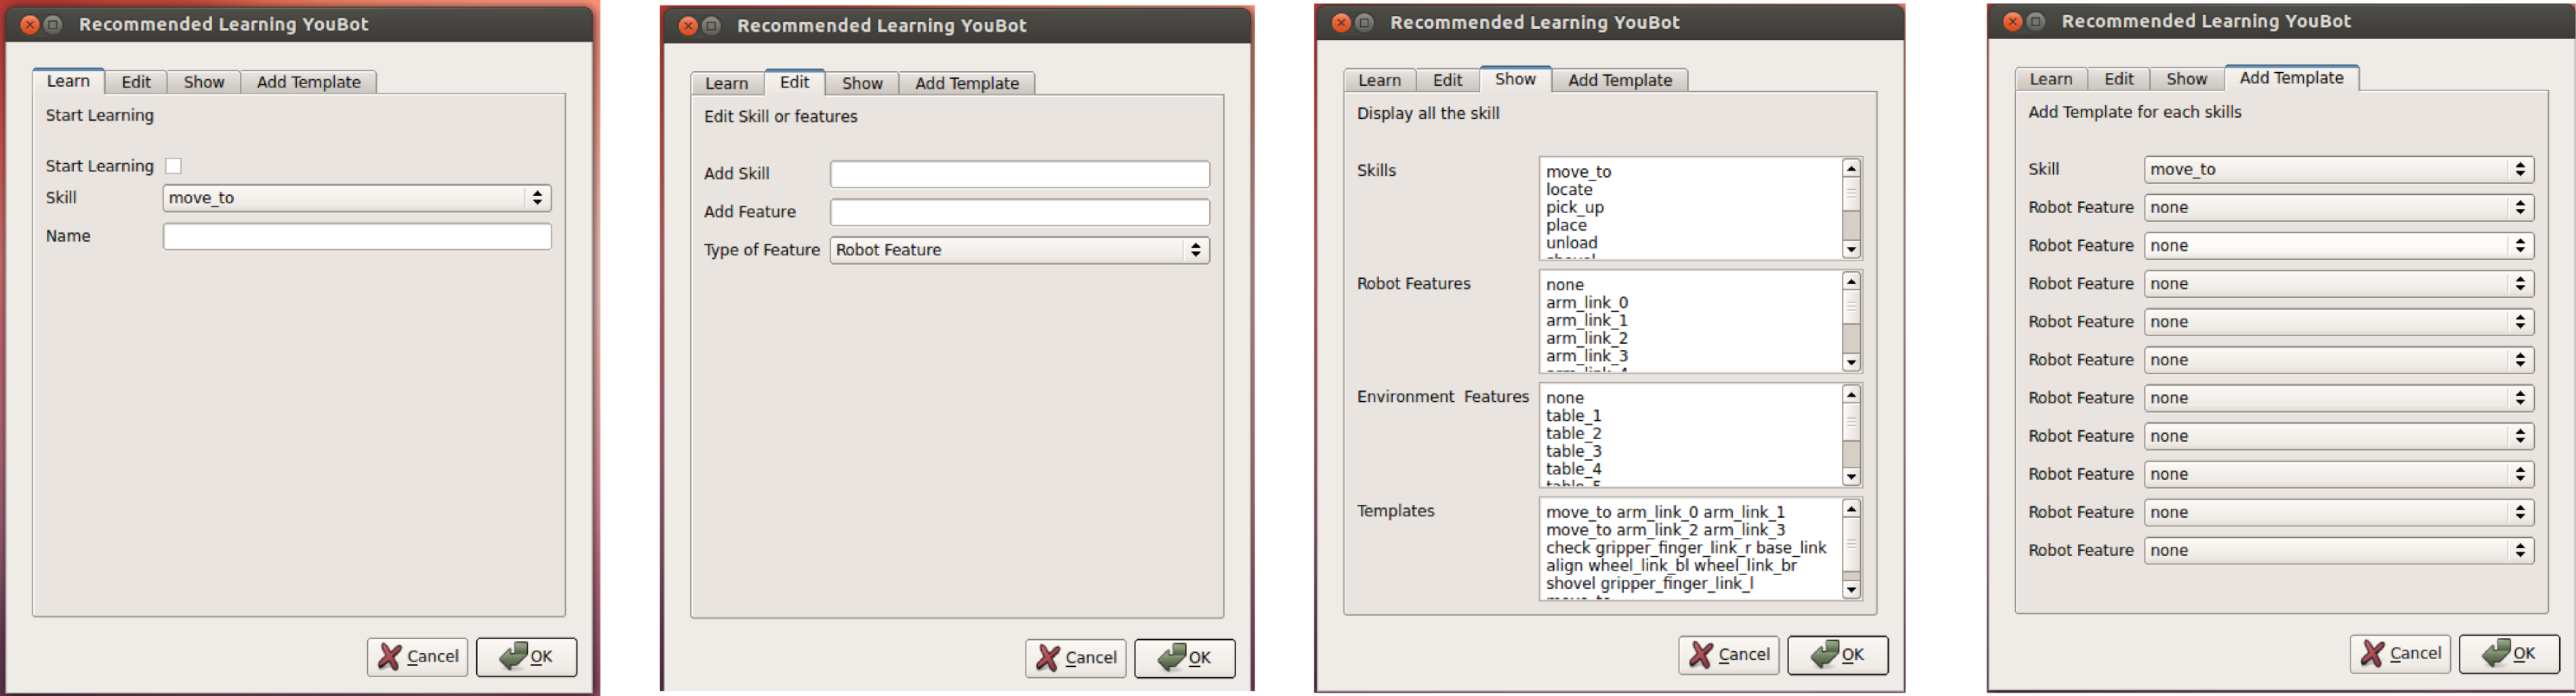
\includegraphics[scale=0.5]{images/tool/tool.png}
\caption[Tool for generating knowledge base]{Tool for generating knowledge base. 1) window for learning a new skill
2) window for editing skill or features 3) Display all features, skills and
templates 4) adding new templates}
\label{}
\end{figure}

On of the limitations of the current efforts in \acrshort{lfd} is adding new features for
new task \cite {argall_survey_2009}. Due to the intuitive nature of
demonstration, \acrshort{lfd} algorithms have the potential to make robot programming
accessible for everyday users who have no programming experience and want to
customize robot behaviours. The use of current approaches by the researchers
, however, is likely to lead to situations in which users attempt to
teach the robot tasks that cannot be learned simply due to the lack of features
describing some aspect of the task.

The solution to such an attempt would be have good tool where the user on 
identification of new features can add new features to the system on which 
the robot can learn.

Also the template creation is an actively changing scenario with various permutations
and combinations possible. The above mentioned tool can be used for rapid 
generation and modification of the templates.


\newpage
\section{Use of Recommender system in robotics}
We started our work based on the notion of using Recommender system in the 
field of robotics. We could partially use the notion of recommender system 
in our work. In the time period of the research various other fields where
the recommender system could be used were identified.
This section list some of the fields of robotics in which technology of 
recommender system fits appropriately.

\subsection{Preferences of users in Task Planing}
With the rise of service robotics in home environments, 
personalized task planning is emerging as a new field of interest.
The robots has to learn the user preferences based on its experience 
with the user and able to modify its decisions regularly.
A common example would be suppose if a user asks the robot for a cup of 
tea, the robot has to make a decision on which cup would be an appropriate 
choice for the user. This choice of the user can be learnt using 
recommender systems.
Works by \cite{abdo_learning_2013} and \cite{abdo_robot_2015} have already 
made progress in this field by using crowd sourcing data.

\subsection{Kernel Recommendation in learning algorithms}
"Firstly, linearity is rather special, and outside quantum mechanics no
model of a real system is truly linear. Secondly, detecting linear
relations has been the focus of much research in statistics and machine
learning for decades and the resulting algorithms are well understood, well
developed and efficient. Naturally, one wants the best of both worlds. So, if a
problem is non-linear, instead of trying to fit a non-linear model, one can map
the problem from the input space to a new (higher-dimensional) space (called
the feature space) by doing a non-linear transformation using suitably chosen
basis functions and then use a linear model in the feature space. This is known
as the 'kernel trick'. The linear model in the feature space corresponds to a
non-linear model in the input space. This approach can be used in both
classification and regression problems. The choice of kernel function is
crucial for the success of all kernel algorithms because the kernel constitutes
prior knowledge that is available about a task. Accordingly, there is no free
lunch (see No Free Lunch Theorems) in kernel choice."
\footnote{\url{http://www.svms.org/kernels/}}

Collaborative based recommender system can be used to determine the kernel 
for learning algorithms. This problem is similar to the n-bandit problem where
the user has to decide on which kernel to keep the bet.

\cite{matikainen_multi-armed_2013} tried to solve the n-bandit problem to
determine which state machine gives better coverage of the floor.
Similar attempts can be made in learning the kernel .

\subsection{Motion Path Planning algorithms }
\acrfull{ompl} has implemented the following planners \url{http://ompl.kavrakilab.org/planners.html}
The selection of the planner for a particular tasks is active scientific 
problem.
If you use the \acrshort{ompl} control , then \acrshort{ompl} will automatically select an
appropriate planner (unless you have explicitly specified one).
If the state
space has a default projection (which is going to be the case if you use any of
the built-in state spaces), then it will use \acrfull{kpiece}. This planner has been
shown to work well consistently across many real-world motion planning
problems, which is why it is the default choice.
In case the state space has no
default projection, \acrfull{rrt} will be used. 
Can we recommend which planner to use in which situation based on previous 
knowledge of the planner in similar situations.
Content based recommender system can be used in such situations to determine 
which planner will be suitable in current situation.

\subsection{Learning trajectory preference of users}
\cite{jain_learning_2013} have worked on learning the trajectory preferences 
of users by on-line learning their feedbacks.
Similar approach can be used as a recommender system to learn 
the user preference of a trajectory for doing a particular tasks.

\newpage
\section{Softwares and tools}

A software implementation and number of tools have been included in the attached
$CD\-ROM$. The tools and the software developed as part of the project.
Below is a brief description of the packages

\begin{itemize}

    \item \textbf{Recommender Learning} \\
        Python based implementation of the learning approach. The class has to be 
        invoked with the folder containing the JSON file of the demonstrations.
        The JSON file is read and learning is made on base of the demonstrations.
        It also reads the knowledge base and creates the set of templates.
        It implements the approach mentioned in section \ref{sec:Learning motion primitive}.
        Available online : \url{https://github.com/deebuls/RecommenderSystemInRobotics/tree/master/code/recommended\_learning}

    \item \textbf{mir\_teleop\_record} \\
        ROS node for teleoperation of the youbot arm and the base. The node was 
        an extension of the work of b-it bots team \url{https://github.com/mas-group/robocup-at-work/tree/brazil-2014/mas\_common\_robotics/mcr\_tools/mcr\_teleop}.
        The node was modified to record the features and to create a JSON file with the readings.
        Available online : \url {https://github.com/deebuls/RecommenderSystemInRobotics/tree/master/code/mir\_teleop\_record }

    \item \textbf{Data accumulator} \\
        The python script for accumulating all the recorded json file and creating
        a consolidated JSON file of the demonstration.
        Available online : \url{https://github.com/deebuls/RecommenderSystemInRobotics/tree/master/code/tools }

    \item \textbf{Knowledge base creator} \\
        An interactive online tool for creating of the knowledge base.
        Menu driven GUI for active interaction with the user and easy to use
        template creation for the knowledge base.
        Available online : \url{ https://github.com/deebuls/RecommenderSystemInRobotics/tree/master/code/knowledge\_base\_creator}

\end{itemize}
